\documentclass[twoside]{book}

% Packages required by doxygen
\usepackage{fixltx2e}
\usepackage{calc}
\usepackage{doxygen}
\usepackage[export]{adjustbox} % also loads graphicx
\usepackage{graphicx}
\usepackage[utf8]{inputenc}
\usepackage{makeidx}
\usepackage{multicol}
\usepackage{multirow}
\PassOptionsToPackage{warn}{textcomp}
\usepackage{textcomp}
\usepackage[nointegrals]{wasysym}
\usepackage[table]{xcolor}

% Font selection
\usepackage[T1]{fontenc}
\usepackage[scaled=.90]{helvet}
\usepackage{courier}
\usepackage{amssymb}
\usepackage{sectsty}
\renewcommand{\familydefault}{\sfdefault}
\allsectionsfont{%
  \fontseries{bc}\selectfont%
  \color{darkgray}%
}
\renewcommand{\DoxyLabelFont}{%
  \fontseries{bc}\selectfont%
  \color{darkgray}%
}
\newcommand{\+}{\discretionary{\mbox{\scriptsize$\hookleftarrow$}}{}{}}

% Page & text layout
\usepackage{geometry}
\geometry{%
  a4paper,%
  top=2.5cm,%
  bottom=2.5cm,%
  left=2.5cm,%
  right=2.5cm%
}
\tolerance=750
\hfuzz=15pt
\hbadness=750
\setlength{\emergencystretch}{15pt}
\setlength{\parindent}{0cm}
\setlength{\parskip}{3ex plus 2ex minus 2ex}
\makeatletter
\renewcommand{\paragraph}{%
  \@startsection{paragraph}{4}{0ex}{-1.0ex}{1.0ex}{%
    \normalfont\normalsize\bfseries\SS@parafont%
  }%
}
\renewcommand{\subparagraph}{%
  \@startsection{subparagraph}{5}{0ex}{-1.0ex}{1.0ex}{%
    \normalfont\normalsize\bfseries\SS@subparafont%
  }%
}
\makeatother

% Headers & footers
\usepackage{fancyhdr}
\pagestyle{fancyplain}
\fancyhead[LE]{\fancyplain{}{\bfseries\thepage}}
\fancyhead[CE]{\fancyplain{}{}}
\fancyhead[RE]{\fancyplain{}{\bfseries\leftmark}}
\fancyhead[LO]{\fancyplain{}{\bfseries\rightmark}}
\fancyhead[CO]{\fancyplain{}{}}
\fancyhead[RO]{\fancyplain{}{\bfseries\thepage}}
\fancyfoot[LE]{\fancyplain{}{}}
\fancyfoot[CE]{\fancyplain{}{}}
\fancyfoot[RE]{\fancyplain{}{\bfseries\scriptsize Generated by Doxygen }}
\fancyfoot[LO]{\fancyplain{}{\bfseries\scriptsize Generated by Doxygen }}
\fancyfoot[CO]{\fancyplain{}{}}
\fancyfoot[RO]{\fancyplain{}{}}
\renewcommand{\footrulewidth}{0.4pt}
\renewcommand{\chaptermark}[1]{%
  \markboth{#1}{}%
}
\renewcommand{\sectionmark}[1]{%
  \markright{\thesection\ #1}%
}

% Indices & bibliography
\usepackage{natbib}
\usepackage[titles]{tocloft}
\setcounter{tocdepth}{3}
\setcounter{secnumdepth}{5}
\makeindex

% Hyperlinks (required, but should be loaded last)
\usepackage{ifpdf}
\ifpdf
  \usepackage[pdftex,pagebackref=true]{hyperref}
\else
  \usepackage[ps2pdf,pagebackref=true]{hyperref}
\fi
\hypersetup{%
  colorlinks=true,%
  linkcolor=blue,%
  citecolor=blue,%
  unicode%
}

% Custom commands
\newcommand{\clearemptydoublepage}{%
  \newpage{\pagestyle{empty}\cleardoublepage}%
}

\usepackage{caption}
\captionsetup{labelsep=space,justification=centering,font={bf},singlelinecheck=off,skip=4pt,position=top}

%===== C O N T E N T S =====

\begin{document}

% Titlepage & ToC
\hypersetup{pageanchor=false,
             bookmarksnumbered=true,
             pdfencoding=unicode
            }
\pagenumbering{alph}
\begin{titlepage}
\vspace*{7cm}
\begin{center}%
{\Large Auris \\[1ex]\large 0.\+1 }\\
\vspace*{1cm}
{\large Generated by Doxygen 1.8.13}\\
\end{center}
\end{titlepage}
\clearemptydoublepage
\pagenumbering{roman}
\tableofcontents
\clearemptydoublepage
\pagenumbering{arabic}
\hypersetup{pageanchor=true}

%--- Begin generated contents ---
\chapter{Hierarchical Index}
\section{Class Hierarchy}
This inheritance list is sorted roughly, but not completely, alphabetically\+:\begin{DoxyCompactList}
\item Audio\+I\+O\+Device\+Callback\begin{DoxyCompactList}
\item \contentsline{section}{Binaural\+Audio\+Source}{\pageref{class_binaural_audio_source}}{}
\end{DoxyCompactList}
\item Component\begin{DoxyCompactList}
\item \contentsline{section}{Main\+Display}{\pageref{class_main_display}}{}
\end{DoxyCompactList}
\item \contentsline{section}{F\+F\+T\+Convolver}{\pageref{class_f_f_t_convolver}}{}
\item \contentsline{section}{F\+P\+S\+Camera}{\pageref{class_f_p_s_camera}}{}
\item \contentsline{section}{H\+R\+T\+F\+Container}{\pageref{class_h_r_t_f_container}}{}
\item \contentsline{section}{Intersection\+Info}{\pageref{struct_intersection_info}}{}
\item \contentsline{section}{Matrix4}{\pageref{class_matrix4}}{}
\item \contentsline{section}{Ray}{\pageref{class_ray}}{}
\item \contentsline{section}{Room}{\pageref{class_room}}{}
\item \contentsline{section}{Sound\+Source}{\pageref{class_sound_source}}{}
\item \contentsline{section}{Sphere}{\pageref{class_sphere}}{}
\item \contentsline{section}{Triangle}{\pageref{class_triangle}}{}
\item \contentsline{section}{Vec3f}{\pageref{struct_vec3f}}{}
\end{DoxyCompactList}

\chapter{Class Index}
\section{Class List}
Here are the classes, structs, unions and interfaces with brief descriptions\+:\begin{DoxyCompactList}
\item\contentsline{section}{\hyperlink{class_binaural_audio_source}{Binaural\+Audio\+Source} }{\pageref{class_binaural_audio_source}}{}
\item\contentsline{section}{\hyperlink{class_f_f_t_convolver}{F\+F\+T\+Convolver} \\*Implementation of a partitioned F\+FT convolution algorithm with uniform block size }{\pageref{class_f_f_t_convolver}}{}
\item\contentsline{section}{\hyperlink{class_f_p_s_camera}{F\+P\+S\+Camera} }{\pageref{class_f_p_s_camera}}{}
\item\contentsline{section}{\hyperlink{class_h_r_t_f_container}{H\+R\+T\+F\+Container} }{\pageref{class_h_r_t_f_container}}{}
\item\contentsline{section}{\hyperlink{struct_intersection_info}{Intersection\+Info} }{\pageref{struct_intersection_info}}{}
\item\contentsline{section}{\hyperlink{class_main_display}{Main\+Display} }{\pageref{class_main_display}}{}
\item\contentsline{section}{\hyperlink{class_matrix4}{Matrix4} }{\pageref{class_matrix4}}{}
\item\contentsline{section}{\hyperlink{class_ray}{Ray} }{\pageref{class_ray}}{}
\item\contentsline{section}{\hyperlink{class_room}{Room} }{\pageref{class_room}}{}
\item\contentsline{section}{\hyperlink{class_sound_source}{Sound\+Source} }{\pageref{class_sound_source}}{}
\item\contentsline{section}{\hyperlink{class_sphere}{Sphere} }{\pageref{class_sphere}}{}
\item\contentsline{section}{\hyperlink{class_triangle}{Triangle} }{\pageref{class_triangle}}{}
\item\contentsline{section}{\hyperlink{struct_vec3f}{Vec3f} }{\pageref{struct_vec3f}}{}
\end{DoxyCompactList}

\chapter{Class Documentation}
\hypertarget{class_binaural_audio_source}{}\section{Binaural\+Audio\+Source Class Reference}
\label{class_binaural_audio_source}\index{Binaural\+Audio\+Source@{Binaural\+Audio\+Source}}
Inheritance diagram for Binaural\+Audio\+Source\+:\begin{figure}[H]
\begin{center}
\leavevmode
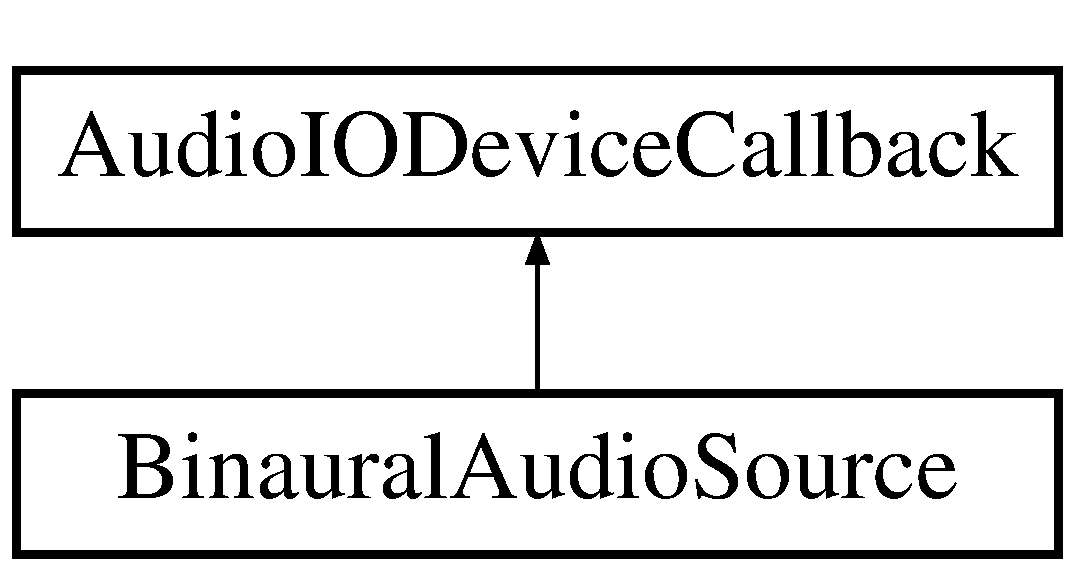
\includegraphics[height=2.000000cm]{class_binaural_audio_source}
\end{center}
\end{figure}
\subsection*{Public Member Functions}
\begin{DoxyCompactItemize}
\item 
\mbox{\Hypertarget{class_binaural_audio_source_a272dd293de333d9f2900b1b827246179}\label{class_binaural_audio_source_a272dd293de333d9f2900b1b827246179}} 
void {\bfseries audio\+Device\+I\+O\+Callback} (const float $\ast$$\ast$input\+Channel\+Data, int total\+Num\+Input\+Channels, float $\ast$$\ast$output\+Channel\+Data, int total\+Num\+Output\+Channels, int num\+Samples)
\item 
\mbox{\Hypertarget{class_binaural_audio_source_a867da6369c0e66c3f7421acfe0bb29b3}\label{class_binaural_audio_source_a867da6369c0e66c3f7421acfe0bb29b3}} 
void {\bfseries audio\+Device\+About\+To\+Start} (Audio\+I\+O\+Device $\ast$device)
\item 
\mbox{\Hypertarget{class_binaural_audio_source_ade028ab523ac34018ca10dc8b0997af5}\label{class_binaural_audio_source_ade028ab523ac34018ca10dc8b0997af5}} 
void {\bfseries audio\+Device\+Stopped} ()
\item 
\mbox{\Hypertarget{class_binaural_audio_source_a946fce5ee9b3cf73df1f8512f7b1485d}\label{class_binaural_audio_source_a946fce5ee9b3cf73df1f8512f7b1485d}} 
void {\bfseries set\+File} (File audio\+File)
\item 
\mbox{\Hypertarget{class_binaural_audio_source_af30ff2e42983e0156cd52c7cf76bf850}\label{class_binaural_audio_source_af30ff2e42983e0156cd52c7cf76bf850}} 
void {\bfseries play} ()
\item 
\mbox{\Hypertarget{class_binaural_audio_source_adad278c8c6e1a24f2209841d589e3ae3}\label{class_binaural_audio_source_adad278c8c6e1a24f2209841d589e3ae3}} 
void {\bfseries set\+Azimuth} (int azimuth)
\item 
\mbox{\Hypertarget{class_binaural_audio_source_a32e840e842c20af332be539066d41a59}\label{class_binaural_audio_source_a32e840e842c20af332be539066d41a59}} 
void {\bfseries set\+Elevation} (int elevation)
\item 
\mbox{\Hypertarget{class_binaural_audio_source_a26cee098b2d2645ce7f4d34df29fb25b}\label{class_binaural_audio_source_a26cee098b2d2645ce7f4d34df29fb25b}} 
void {\bfseries update\+H\+R\+IR} (double azimuth, double elevation)
\item 
\mbox{\Hypertarget{class_binaural_audio_source_a1f3a74e7a1905ebdd60c2bcc221bc3b6}\label{class_binaural_audio_source_a1f3a74e7a1905ebdd60c2bcc221bc3b6}} 
void {\bfseries bypass\+Audio} (bool is\+Bypassed)
\item 
\mbox{\Hypertarget{class_binaural_audio_source_a009b7bc8cfd9ea4c5030035de1550d18}\label{class_binaural_audio_source_a009b7bc8cfd9ea4c5030035de1550d18}} 
void {\bfseries set\+Distance} (int distance)
\end{DoxyCompactItemize}


The documentation for this class was generated from the following file\+:\begin{DoxyCompactItemize}
\item 
Audio/Binaural\+Audio\+Source.\+h\end{DoxyCompactItemize}

\hypertarget{class_f_f_t_convolver}{}\section{F\+F\+T\+Convolver Class Reference}
\label{class_f_f_t_convolver}\index{F\+F\+T\+Convolver@{F\+F\+T\+Convolver}}


Implementation of a partitioned F\+FT convolution algorithm with uniform block size.  




{\ttfamily \#include $<$F\+F\+T\+Convolver.\+h$>$}

\subsection*{Public Member Functions}
\begin{DoxyCompactItemize}
\item 
void \hyperlink{class_f_f_t_convolver_a7cd43a369a1c2064c2e360d11287f41b}{init} (unsigned long block\+Size, const float $\ast$ir, unsigned long ir\+Len)
\begin{DoxyCompactList}\small\item\em Initializes the convolver. \end{DoxyCompactList}\item 
void \hyperlink{class_f_f_t_convolver_a31b560596aea14e50ad48bde70571665}{process} (const float $\ast$input, float $\ast$output, size\+\_\+t len)
\begin{DoxyCompactList}\small\item\em Convolves the the given input floats and immediately outputs the result. \end{DoxyCompactList}\item 
\mbox{\Hypertarget{class_f_f_t_convolver_a31e77811a5c845d3639a0c41634eb792}\label{class_f_f_t_convolver_a31e77811a5c845d3639a0c41634eb792}} 
void \hyperlink{class_f_f_t_convolver_a31e77811a5c845d3639a0c41634eb792}{reset} ()
\begin{DoxyCompactList}\small\item\em Resets the convolver and discards the set impulse response. \end{DoxyCompactList}\item 
\mbox{\Hypertarget{class_f_f_t_convolver_ac7cb580fadccfcdbeca7a7fd81817245}\label{class_f_f_t_convolver_ac7cb580fadccfcdbeca7a7fd81817245}} 
void {\bfseries set\+IR} (const float $\ast$ir)
\end{DoxyCompactItemize}


\subsection{Detailed Description}
Implementation of a partitioned F\+FT convolution algorithm with uniform block size. 

Some notes on how to use it\+:


\begin{DoxyItemize}
\item After initialization with an impulse response, subsequent data portions of arbitrary length can be convolved. The convolver internally can handle this by using appropriate buffering.
\item The convolver works without \char`\"{}latency\char`\"{} (except for the required processing time, of course), i.\+e. the output always is the convolved input for each processing call.
\item The convolver is suitable for real-\/time processing which means that no \char`\"{}unpredictable\char`\"{} operations like allocations, locking, A\+PI calls, etc. are performed during processing (all necessary allocations and preparations take place during initialization). 
\end{DoxyItemize}

\subsection{Member Function Documentation}
\mbox{\Hypertarget{class_f_f_t_convolver_a7cd43a369a1c2064c2e360d11287f41b}\label{class_f_f_t_convolver_a7cd43a369a1c2064c2e360d11287f41b}} 
\index{F\+F\+T\+Convolver@{F\+F\+T\+Convolver}!init@{init}}
\index{init@{init}!F\+F\+T\+Convolver@{F\+F\+T\+Convolver}}
\subsubsection{\texorpdfstring{init()}{init()}}
{\footnotesize\ttfamily void F\+F\+T\+Convolver\+::init (\begin{DoxyParamCaption}\item[{unsigned long}]{block\+Size,  }\item[{const float $\ast$}]{ir,  }\item[{unsigned long}]{ir\+Len }\end{DoxyParamCaption})}



Initializes the convolver. 


\begin{DoxyParams}{Parameters}
{\em block\+Size} & Block size internally used by the convolver (partition size) \\
\hline
{\em ir} & The impulse response \\
\hline
{\em ir\+Len} & Length of the impulse response \\
\hline
\end{DoxyParams}
\begin{DoxyReturn}{Returns}
true\+: Success -\/ false\+: Failed 
\end{DoxyReturn}
\mbox{\Hypertarget{class_f_f_t_convolver_a31b560596aea14e50ad48bde70571665}\label{class_f_f_t_convolver_a31b560596aea14e50ad48bde70571665}} 
\index{F\+F\+T\+Convolver@{F\+F\+T\+Convolver}!process@{process}}
\index{process@{process}!F\+F\+T\+Convolver@{F\+F\+T\+Convolver}}
\subsubsection{\texorpdfstring{process()}{process()}}
{\footnotesize\ttfamily void F\+F\+T\+Convolver\+::process (\begin{DoxyParamCaption}\item[{const float $\ast$}]{input,  }\item[{float $\ast$}]{output,  }\item[{size\+\_\+t}]{len }\end{DoxyParamCaption})}



Convolves the the given input floats and immediately outputs the result. 


\begin{DoxyParams}{Parameters}
{\em input} & The input floats \\
\hline
{\em output} & The convolution result \\
\hline
{\em len} & Number of input/output floats \\
\hline
\end{DoxyParams}


The documentation for this class was generated from the following file\+:\begin{DoxyCompactItemize}
\item 
Audio/\+F\+F\+T\+Convolver/F\+F\+T\+Convolver.\+h\end{DoxyCompactItemize}

\hypertarget{class_f_p_s_camera}{}\section{F\+P\+S\+Camera Class Reference}
\label{class_f_p_s_camera}\index{F\+P\+S\+Camera@{F\+P\+S\+Camera}}
\subsection*{Public Member Functions}
\begin{DoxyCompactItemize}
\item 
\mbox{\Hypertarget{class_f_p_s_camera_a3559b2ac359911c6e5dd9449fda72082}\label{class_f_p_s_camera_a3559b2ac359911c6e5dd9449fda72082}} 
\hyperlink{struct_vec3f}{Vec3f} {\bfseries get\+Position} ()
\item 
\mbox{\Hypertarget{class_f_p_s_camera_a8e0c8ebfc81b01e542e9b2972c8562c1}\label{class_f_p_s_camera_a8e0c8ebfc81b01e542e9b2972c8562c1}} 
\hyperlink{struct_vec3f}{Vec3f} {\bfseries get\+View} ()
\item 
\mbox{\Hypertarget{class_f_p_s_camera_a05857c6e4262f11e83d2cf824b161b0e}\label{class_f_p_s_camera_a05857c6e4262f11e83d2cf824b161b0e}} 
\hyperlink{struct_vec3f}{Vec3f} {\bfseries get\+Up\+Vector} ()
\item 
\mbox{\Hypertarget{class_f_p_s_camera_a131adcf4cdb53546900583556dae0071}\label{class_f_p_s_camera_a131adcf4cdb53546900583556dae0071}} 
\hyperlink{struct_vec3f}{Vec3f} {\bfseries get\+Strafe} ()
\item 
\mbox{\Hypertarget{class_f_p_s_camera_a96fdf7fc079dea4aa9c360e195ec9bc9}\label{class_f_p_s_camera_a96fdf7fc079dea4aa9c360e195ec9bc9}} 
\hyperlink{class_sphere}{Sphere} {\bfseries get\+Collison\+Sphere} ()
\item 
\mbox{\Hypertarget{class_f_p_s_camera_a00fbb3eac9d77b41ccc71a67df9a6716}\label{class_f_p_s_camera_a00fbb3eac9d77b41ccc71a67df9a6716}} 
float {\bfseries get\+Xrotation} ()
\item 
\mbox{\Hypertarget{class_f_p_s_camera_ab2fb3b866d0e0c545f6366769e8530fc}\label{class_f_p_s_camera_ab2fb3b866d0e0c545f6366769e8530fc}} 
float {\bfseries get\+Yrotation} ()
\item 
\mbox{\Hypertarget{class_f_p_s_camera_a3c6d11e5ad8c8417c5ad9be0d97cf4d6}\label{class_f_p_s_camera_a3c6d11e5ad8c8417c5ad9be0d97cf4d6}} 
void {\bfseries set\+Position} (float positionX, float positionY, float positionZ, float viewX, float viewY, float viewZ, float up\+VectorX, float up\+VectorY, float up\+VectorZ)
\item 
\mbox{\Hypertarget{class_f_p_s_camera_a7a4ade212677a3f6da321f1dea7ab572}\label{class_f_p_s_camera_a7a4ade212677a3f6da321f1dea7ab572}} 
void {\bfseries rotate\+View} (float angle, float X, float Y, float Z)
\item 
\mbox{\Hypertarget{class_f_p_s_camera_ae596d38d60db97bdf617d5f2cfade10b}\label{class_f_p_s_camera_ae596d38d60db97bdf617d5f2cfade10b}} 
void {\bfseries set\+View\+By\+Mouse} (float mouseX, float mouseY, int width, int height)
\item 
\mbox{\Hypertarget{class_f_p_s_camera_aeddf4e5206e4c2f4ef44bc7cbcb68776}\label{class_f_p_s_camera_aeddf4e5206e4c2f4ef44bc7cbcb68776}} 
void {\bfseries rotate\+Around\+Point} (\hyperlink{struct_vec3f}{Vec3f} v\+Center, float X, float Y, float Z)
\item 
\mbox{\Hypertarget{class_f_p_s_camera_a5dfb63b3f68c9682444011b60c1c998c}\label{class_f_p_s_camera_a5dfb63b3f68c9682444011b60c1c998c}} 
void {\bfseries set\+Xrotation} (float rotation)
\item 
\mbox{\Hypertarget{class_f_p_s_camera_a6298cea0150128aab9b71db46b33c7b6}\label{class_f_p_s_camera_a6298cea0150128aab9b71db46b33c7b6}} 
void {\bfseries strafe} (float speed)
\item 
\mbox{\Hypertarget{class_f_p_s_camera_a6a0cac90ac9fcfaef12fe16bad8ed24d}\label{class_f_p_s_camera_a6a0cac90ac9fcfaef12fe16bad8ed24d}} 
void {\bfseries move} (float speed)
\item 
\mbox{\Hypertarget{class_f_p_s_camera_a1792fa28fa33dd6efda48f13b7b610dd}\label{class_f_p_s_camera_a1792fa28fa33dd6efda48f13b7b610dd}} 
void {\bfseries check\+For\+Movement} ()
\item 
\mbox{\Hypertarget{class_f_p_s_camera_a738560c0c908cf654776cbad1264e493}\label{class_f_p_s_camera_a738560c0c908cf654776cbad1264e493}} 
void {\bfseries update} (float mouseX, float mouseY, int width, int height)
\item 
\mbox{\Hypertarget{class_f_p_s_camera_a2ccca2c82f14e38b4fd32875a7e9da25}\label{class_f_p_s_camera_a2ccca2c82f14e38b4fd32875a7e9da25}} 
void {\bfseries look} ()
\item 
\mbox{\Hypertarget{class_f_p_s_camera_a503e4704b8858062f10e7aedd091d3c9}\label{class_f_p_s_camera_a503e4704b8858062f10e7aedd091d3c9}} 
void {\bfseries check\+Camera\+Collision} (\hyperlink{class_triangle}{Triangle} $\ast$room\+Triangles, int num\+Triangles)
\item 
\mbox{\Hypertarget{class_f_p_s_camera_a32904ec6c5592810188db68cd9c13a52}\label{class_f_p_s_camera_a32904ec6c5592810188db68cd9c13a52}} 
\hyperlink{struct_vec3f}{Vec3f} {\bfseries get\+Collision\+Offset} (\hyperlink{struct_vec3f}{Vec3f} \&v\+Normal, float radius, float distance)
\end{DoxyCompactItemize}
\subsection*{Public Attributes}
\begin{DoxyCompactItemize}
\item 
\mbox{\Hypertarget{class_f_p_s_camera_ae33a5225fc7cab505ba74bb4d0df4b99}\label{class_f_p_s_camera_ae33a5225fc7cab505ba74bb4d0df4b99}} 
\hyperlink{class_sphere}{Sphere} {\bfseries sphere}
\end{DoxyCompactItemize}


The documentation for this class was generated from the following file\+:\begin{DoxyCompactItemize}
\item 
Camera/Camera.\+h\end{DoxyCompactItemize}

\hypertarget{class_h_r_t_f_container}{}\section{H\+R\+T\+F\+Container Class Reference}
\label{class_h_r_t_f_container}\index{H\+R\+T\+F\+Container@{H\+R\+T\+F\+Container}}
\subsection*{Public Member Functions}
\begin{DoxyCompactItemize}
\item 
\mbox{\Hypertarget{class_h_r_t_f_container_aa161195100a640db166f5f97a71ec24a}\label{class_h_r_t_f_container_aa161195100a640db166f5f97a71ec24a}} 
void {\bfseries update\+H\+R\+IR} (double azimuth, double elevation)
\item 
\mbox{\Hypertarget{class_h_r_t_f_container_ad046e3424e66a7245062e92288dc2375}\label{class_h_r_t_f_container_ad046e3424e66a7245062e92288dc2375}} 
const Hrir\+Buffer \& {\bfseries hrir} () const
\end{DoxyCompactItemize}
\subsection*{Public Attributes}
\begin{DoxyCompactItemize}
\item 
\mbox{\Hypertarget{class_h_r_t_f_container_a675fdb70347737917fe1f2431f38a5f2}\label{class_h_r_t_f_container_a675fdb70347737917fe1f2431f38a5f2}} 
Audio\+Sample\+Buffer {\bfseries left\+Ear}
\item 
\mbox{\Hypertarget{class_h_r_t_f_container_afd9732627ecdbf70dde9d37b9d7f28a4}\label{class_h_r_t_f_container_afd9732627ecdbf70dde9d37b9d7f28a4}} 
Audio\+Sample\+Buffer {\bfseries right\+Ear}
\item 
\mbox{\Hypertarget{class_h_r_t_f_container_a53ae96c68982ce8b7a736872d1f55fbc}\label{class_h_r_t_f_container_a53ae96c68982ce8b7a736872d1f55fbc}} 
Hrir\+Buffer {\bfseries hrir\+\_\+}
\end{DoxyCompactItemize}


The documentation for this class was generated from the following file\+:\begin{DoxyCompactItemize}
\item 
Audio/H\+R\+T\+F\+Container.\+h\end{DoxyCompactItemize}

\hypertarget{struct_intersection_info}{}\section{Intersection\+Info Struct Reference}
\label{struct_intersection_info}\index{Intersection\+Info@{Intersection\+Info}}
\subsection*{Public Attributes}
\begin{DoxyCompactItemize}
\item 
\mbox{\Hypertarget{struct_intersection_info_a44961e762372a8b82d7df4b8b26d02fd}\label{struct_intersection_info_a44961e762372a8b82d7df4b8b26d02fd}} 
\hyperlink{class_sphere}{Sphere} $\ast$ {\bfseries object}
\item 
\mbox{\Hypertarget{struct_intersection_info_a981e179dbf67e4d511b36f6704f812a7}\label{struct_intersection_info_a981e179dbf67e4d511b36f6704f812a7}} 
\hyperlink{struct_vec3f}{Vec3f} {\bfseries inters\+Point}
\item 
\mbox{\Hypertarget{struct_intersection_info_af4044613d62580c855b795b1a5789a37}\label{struct_intersection_info_af4044613d62580c855b795b1a5789a37}} 
float {\bfseries distance}
\end{DoxyCompactItemize}


The documentation for this struct was generated from the following file\+:\begin{DoxyCompactItemize}
\item 
Primitives/Intersection\+Info.\+h\end{DoxyCompactItemize}

\hypertarget{class_main_display}{}\section{Main\+Display Class Reference}
\label{class_main_display}\index{Main\+Display@{Main\+Display}}
Inheritance diagram for Main\+Display\+:\begin{figure}[H]
\begin{center}
\leavevmode
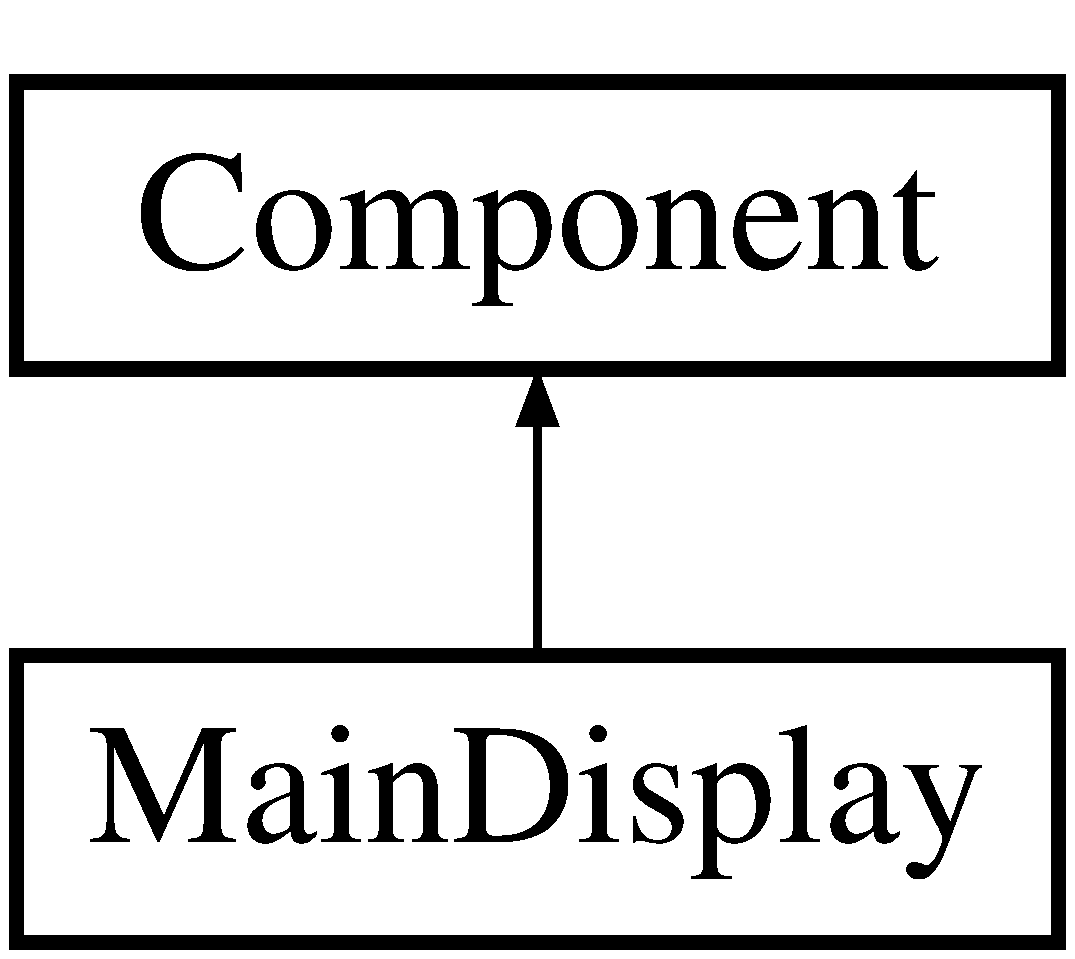
\includegraphics[height=2.000000cm]{class_main_display}
\end{center}
\end{figure}
\subsection*{Public Member Functions}
\begin{DoxyCompactItemize}
\item 
\mbox{\Hypertarget{class_main_display_a400f3f47e5251a4a0ba5396fb8c1bd7a}\label{class_main_display_a400f3f47e5251a4a0ba5396fb8c1bd7a}} 
void {\bfseries paint} (Graphics \&g) override
\item 
\mbox{\Hypertarget{class_main_display_a66c6000e605709fe14f3395a9487900c}\label{class_main_display_a66c6000e605709fe14f3395a9487900c}} 
void {\bfseries set\+Sources} (std\+::vector$<$ Scoped\+Pointer$<$ \hyperlink{class_sound_source}{Sound\+Source} $>$$>$ $\ast$sources)
\end{DoxyCompactItemize}


The documentation for this class was generated from the following file\+:\begin{DoxyCompactItemize}
\item 
Component/Main\+Display.\+h\end{DoxyCompactItemize}

\hypertarget{class_matrix4}{}\section{Matrix4 Class Reference}
\label{class_matrix4}\index{Matrix4@{Matrix4}}
\subsection*{Public Member Functions}
\begin{DoxyCompactItemize}
\item 
\mbox{\Hypertarget{class_matrix4_a5aa337a51c2ea4e08bb6fdb46bac4007}\label{class_matrix4_a5aa337a51c2ea4e08bb6fdb46bac4007}} 
{\bfseries Matrix4} (const float src\mbox{[}16\mbox{]})
\item 
\mbox{\Hypertarget{class_matrix4_a79283dde33d6c1eabbafdb9deec41c19}\label{class_matrix4_a79283dde33d6c1eabbafdb9deec41c19}} 
{\bfseries Matrix4} (float xx, float xy, float xz, float xw, float yx, float yy, float yz, float yw, float zx, float zy, float zz, float zw, float wx, float wy, float wz, float ww)
\item 
\mbox{\Hypertarget{class_matrix4_af8b9f45c14e981509d141d00a0d87a6c}\label{class_matrix4_af8b9f45c14e981509d141d00a0d87a6c}} 
void {\bfseries set} (const float src\mbox{[}16\mbox{]})
\item 
\mbox{\Hypertarget{class_matrix4_a043609890084209a0bca280826a987e3}\label{class_matrix4_a043609890084209a0bca280826a987e3}} 
void {\bfseries set} (float xx, float xy, float xz, float xw, float yx, float yy, float yz, float yw, float zx, float zy, float zz, float zw, float wx, float wy, float wz, float ww)
\item 
\mbox{\Hypertarget{class_matrix4_ac516425bfa040853a4bb61ecc0e26d83}\label{class_matrix4_ac516425bfa040853a4bb61ecc0e26d83}} 
void {\bfseries set\+Row} (int index, const float row\mbox{[}4\mbox{]})
\item 
\mbox{\Hypertarget{class_matrix4_a37923fa6fc00df9f3358cf2cae135773}\label{class_matrix4_a37923fa6fc00df9f3358cf2cae135773}} 
void {\bfseries set\+Row} (int index, const \hyperlink{struct_vec3f}{Vec3f} \&v)
\item 
\mbox{\Hypertarget{class_matrix4_ab4fc658fab1f55c57177985114026c60}\label{class_matrix4_ab4fc658fab1f55c57177985114026c60}} 
void {\bfseries set\+Column} (int index, const float col\mbox{[}4\mbox{]})
\item 
\mbox{\Hypertarget{class_matrix4_ad40fe940b9977bf5ee4da8e293d531e8}\label{class_matrix4_ad40fe940b9977bf5ee4da8e293d531e8}} 
void {\bfseries set\+Column} (int index, const \hyperlink{struct_vec3f}{Vec3f} \&v)
\item 
\mbox{\Hypertarget{class_matrix4_a31c109fc6162eb7c5901a8b2a7db14ad}\label{class_matrix4_a31c109fc6162eb7c5901a8b2a7db14ad}} 
const float $\ast$ {\bfseries get} () const
\item 
\mbox{\Hypertarget{class_matrix4_a9914294a87c0974ca6811c43a5127668}\label{class_matrix4_a9914294a87c0974ca6811c43a5127668}} 
const float $\ast$ {\bfseries get\+Transpose} ()
\item 
\mbox{\Hypertarget{class_matrix4_aa4364553435acdea523deae68dc3c27f}\label{class_matrix4_aa4364553435acdea523deae68dc3c27f}} 
float {\bfseries get\+Determinant} ()
\item 
\mbox{\Hypertarget{class_matrix4_a6579c04e6c37890a0f109450457b7d5d}\label{class_matrix4_a6579c04e6c37890a0f109450457b7d5d}} 
\hyperlink{class_matrix4}{Matrix4} \& {\bfseries identity} ()
\item 
\mbox{\Hypertarget{class_matrix4_a71e0b29252a6e3c78e396342ac459e40}\label{class_matrix4_a71e0b29252a6e3c78e396342ac459e40}} 
\hyperlink{class_matrix4}{Matrix4} \& {\bfseries transpose} ()
\item 
\mbox{\Hypertarget{class_matrix4_a47f0c18f047af011ae6f20203d4c67f1}\label{class_matrix4_a47f0c18f047af011ae6f20203d4c67f1}} 
\hyperlink{class_matrix4}{Matrix4} \& {\bfseries invert} ()
\item 
\mbox{\Hypertarget{class_matrix4_a9526c76f1d5872a42f46f7ab14a7b68b}\label{class_matrix4_a9526c76f1d5872a42f46f7ab14a7b68b}} 
\hyperlink{class_matrix4}{Matrix4} \& {\bfseries invert\+Euclidean} ()
\item 
\mbox{\Hypertarget{class_matrix4_a35ce605b965e642413df0ec9f214e8ef}\label{class_matrix4_a35ce605b965e642413df0ec9f214e8ef}} 
\hyperlink{class_matrix4}{Matrix4} \& {\bfseries invert\+Projective} ()
\item 
\mbox{\Hypertarget{class_matrix4_aac71771a4781a04d54091acf710edb55}\label{class_matrix4_aac71771a4781a04d54091acf710edb55}} 
\hyperlink{class_matrix4}{Matrix4} \& {\bfseries invert\+General} ()
\item 
\mbox{\Hypertarget{class_matrix4_ab1c73ac475b67cdf8e6cdc579b0a1bbb}\label{class_matrix4_ab1c73ac475b67cdf8e6cdc579b0a1bbb}} 
\hyperlink{class_matrix4}{Matrix4} \& {\bfseries translate} (float x, float y, float z)
\item 
\mbox{\Hypertarget{class_matrix4_a921da95960136c2a3d35268c439612d8}\label{class_matrix4_a921da95960136c2a3d35268c439612d8}} 
\hyperlink{class_matrix4}{Matrix4} \& {\bfseries translate} (const \hyperlink{struct_vec3f}{Vec3f} \&v)
\item 
\mbox{\Hypertarget{class_matrix4_abef349a41e8700adc382057ba5457fd2}\label{class_matrix4_abef349a41e8700adc382057ba5457fd2}} 
\hyperlink{class_matrix4}{Matrix4} \& {\bfseries rotate} (float angle, const \hyperlink{struct_vec3f}{Vec3f} \&axis)
\item 
\mbox{\Hypertarget{class_matrix4_a34f2e5da0cfd8ddb77579b0c2f1c4255}\label{class_matrix4_a34f2e5da0cfd8ddb77579b0c2f1c4255}} 
\hyperlink{class_matrix4}{Matrix4} \& {\bfseries rotate} (float angle, float x, float y, float z)
\item 
\mbox{\Hypertarget{class_matrix4_a25558cec243bd6d5e94fdc9314f05a9e}\label{class_matrix4_a25558cec243bd6d5e94fdc9314f05a9e}} 
\hyperlink{class_matrix4}{Matrix4} \& {\bfseries rotateX} (float angle)
\item 
\mbox{\Hypertarget{class_matrix4_a8a050af5438b578728b5105ae15f5cfb}\label{class_matrix4_a8a050af5438b578728b5105ae15f5cfb}} 
\hyperlink{class_matrix4}{Matrix4} \& {\bfseries rotateY} (float angle)
\item 
\mbox{\Hypertarget{class_matrix4_ace8f7ee2e56fb5316b21bdcaf4491509}\label{class_matrix4_ace8f7ee2e56fb5316b21bdcaf4491509}} 
\hyperlink{class_matrix4}{Matrix4} \& {\bfseries rotateZ} (float angle)
\item 
\mbox{\Hypertarget{class_matrix4_acade41d13743c554d79e844f43019c23}\label{class_matrix4_acade41d13743c554d79e844f43019c23}} 
\hyperlink{class_matrix4}{Matrix4} \& {\bfseries scale} (float scale)
\item 
\mbox{\Hypertarget{class_matrix4_a28c20caa1f9dcbc77bae379207028a03}\label{class_matrix4_a28c20caa1f9dcbc77bae379207028a03}} 
\hyperlink{class_matrix4}{Matrix4} \& {\bfseries scale} (float sx, float sy, float sz)
\item 
\mbox{\Hypertarget{class_matrix4_a61b8f5a2f89ae56c43b91e750ae6e580}\label{class_matrix4_a61b8f5a2f89ae56c43b91e750ae6e580}} 
\hyperlink{class_matrix4}{Matrix4} {\bfseries operator+} (const \hyperlink{class_matrix4}{Matrix4} \&rhs) const
\item 
\mbox{\Hypertarget{class_matrix4_a8ee3db0a15525fa4cdde282f8b94b7df}\label{class_matrix4_a8ee3db0a15525fa4cdde282f8b94b7df}} 
\hyperlink{class_matrix4}{Matrix4} {\bfseries operator-\/} (const \hyperlink{class_matrix4}{Matrix4} \&rhs) const
\item 
\mbox{\Hypertarget{class_matrix4_aa25858af1530f2c1101349e10cb5ab0d}\label{class_matrix4_aa25858af1530f2c1101349e10cb5ab0d}} 
\hyperlink{class_matrix4}{Matrix4} \& {\bfseries operator+=} (const \hyperlink{class_matrix4}{Matrix4} \&rhs)
\item 
\mbox{\Hypertarget{class_matrix4_a6fe855f09d83716443ab52a59ad87558}\label{class_matrix4_a6fe855f09d83716443ab52a59ad87558}} 
\hyperlink{class_matrix4}{Matrix4} \& {\bfseries operator-\/=} (const \hyperlink{class_matrix4}{Matrix4} \&rhs)
\item 
\mbox{\Hypertarget{class_matrix4_a97881e3beb48b2345cefafd3bc80ab58}\label{class_matrix4_a97881e3beb48b2345cefafd3bc80ab58}} 
\hyperlink{struct_vec3f}{Vec3f} {\bfseries operator$\ast$} (const \hyperlink{struct_vec3f}{Vec3f} \&rhs) const
\item 
\mbox{\Hypertarget{class_matrix4_ace5fb62ba207d9b1ac7ab7a366957f60}\label{class_matrix4_ace5fb62ba207d9b1ac7ab7a366957f60}} 
\hyperlink{class_matrix4}{Matrix4} {\bfseries operator$\ast$} (const \hyperlink{class_matrix4}{Matrix4} \&rhs) const
\item 
\mbox{\Hypertarget{class_matrix4_a86ddf7cab948e73a4a3ec05e7c62158c}\label{class_matrix4_a86ddf7cab948e73a4a3ec05e7c62158c}} 
\hyperlink{class_matrix4}{Matrix4} \& {\bfseries operator$\ast$=} (const \hyperlink{class_matrix4}{Matrix4} \&rhs)
\item 
\mbox{\Hypertarget{class_matrix4_a65f9a69947847a8a4d98faa87746a246}\label{class_matrix4_a65f9a69947847a8a4d98faa87746a246}} 
bool {\bfseries operator==} (const \hyperlink{class_matrix4}{Matrix4} \&rhs) const
\item 
\mbox{\Hypertarget{class_matrix4_ada121f001badf192d7d01c546a752fd0}\label{class_matrix4_ada121f001badf192d7d01c546a752fd0}} 
bool {\bfseries operator!=} (const \hyperlink{class_matrix4}{Matrix4} \&rhs) const
\item 
\mbox{\Hypertarget{class_matrix4_a71baac5e31f0b8e70d40a897d31706dd}\label{class_matrix4_a71baac5e31f0b8e70d40a897d31706dd}} 
float {\bfseries operator\mbox{[}$\,$\mbox{]}} (int index) const
\item 
\mbox{\Hypertarget{class_matrix4_a3e542f89134e7496dfe820ba1668b305}\label{class_matrix4_a3e542f89134e7496dfe820ba1668b305}} 
float \& {\bfseries operator\mbox{[}$\,$\mbox{]}} (int index)
\end{DoxyCompactItemize}
\subsection*{Friends}
\begin{DoxyCompactItemize}
\item 
\mbox{\Hypertarget{class_matrix4_a9d189e964a989207c8489e80276dadd4}\label{class_matrix4_a9d189e964a989207c8489e80276dadd4}} 
\hyperlink{class_matrix4}{Matrix4} {\bfseries operator-\/} (const \hyperlink{class_matrix4}{Matrix4} \&m)
\item 
\mbox{\Hypertarget{class_matrix4_ab1dd86a7d3fd19e91a596c844ba89061}\label{class_matrix4_ab1dd86a7d3fd19e91a596c844ba89061}} 
\hyperlink{class_matrix4}{Matrix4} {\bfseries operator$\ast$} (float scalar, const \hyperlink{class_matrix4}{Matrix4} \&m)
\item 
\mbox{\Hypertarget{class_matrix4_afdc4698112c038343150d1feff5bedb9}\label{class_matrix4_afdc4698112c038343150d1feff5bedb9}} 
\hyperlink{struct_vec3f}{Vec3f} {\bfseries operator$\ast$} (const \hyperlink{struct_vec3f}{Vec3f} \&vec, const \hyperlink{class_matrix4}{Matrix4} \&m)
\end{DoxyCompactItemize}


The documentation for this class was generated from the following file\+:\begin{DoxyCompactItemize}
\item 
Math/Matrices.\+h\end{DoxyCompactItemize}

\hypertarget{class_ray}{}\section{Ray Class Reference}
\label{class_ray}\index{Ray@{Ray}}
\subsection*{Public Member Functions}
\begin{DoxyCompactItemize}
\item 
\mbox{\Hypertarget{class_ray_ac83ad4e3f84ea20a5e198ce490bc3826}\label{class_ray_ac83ad4e3f84ea20a5e198ce490bc3826}} 
{\bfseries Ray} (const \hyperlink{struct_vec3f}{Vec3f} \&start\+Pos, const \hyperlink{struct_vec3f}{Vec3f} \&direction)
\item 
\mbox{\Hypertarget{class_ray_adba75771d6aea287b72ddde4300d3265}\label{class_ray_adba75771d6aea287b72ddde4300d3265}} 
bool {\bfseries intersected\+Plane} (\hyperlink{struct_vec3f}{Vec3f} plane\+Normal, \hyperlink{struct_vec3f}{Vec3f} plane\+Vertex, \hyperlink{struct_vec3f}{Vec3f} \&v\+Normal, float \&origin\+Distance)
\item 
\mbox{\Hypertarget{class_ray_a74730563d54fd38b2fd1beaad71124dd}\label{class_ray_a74730563d54fd38b2fd1beaad71124dd}} 
\hyperlink{struct_vec3f}{Vec3f} {\bfseries get\+Reflection\+Vector} (\hyperlink{struct_vec3f}{Vec3f} plane\+Normal)
\end{DoxyCompactItemize}
\subsection*{Public Attributes}
\begin{DoxyCompactItemize}
\item 
\mbox{\Hypertarget{class_ray_a1cd7e5204c62e055877be67ece18df68}\label{class_ray_a1cd7e5204c62e055877be67ece18df68}} 
\hyperlink{struct_vec3f}{Vec3f} {\bfseries start\+Pos}
\item 
\mbox{\Hypertarget{class_ray_a884ffd8791df6d6613df52c9feb6ee0a}\label{class_ray_a884ffd8791df6d6613df52c9feb6ee0a}} 
\hyperlink{struct_vec3f}{Vec3f} {\bfseries direction}
\end{DoxyCompactItemize}


The documentation for this class was generated from the following file\+:\begin{DoxyCompactItemize}
\item 
Primitives/Ray.\+h\end{DoxyCompactItemize}

\hypertarget{class_room}{}\section{Room Class Reference}
\label{class_room}\index{Room@{Room}}
\subsection*{Public Member Functions}
\begin{DoxyCompactItemize}
\item 
\mbox{\Hypertarget{class_room_a51424a2ca4f39eb25b701c07460cd5bc}\label{class_room_a51424a2ca4f39eb25b701c07460cd5bc}} 
void {\bfseries load} ()
\item 
\mbox{\Hypertarget{class_room_a40aeeb4083bfd0f84c2fc88ec1713230}\label{class_room_a40aeeb4083bfd0f84c2fc88ec1713230}} 
void {\bfseries draw} ()
\item 
\mbox{\Hypertarget{class_room_a6bf70ed9beba2549a90e8dcb9540c019}\label{class_room_a6bf70ed9beba2549a90e8dcb9540c019}} 
int {\bfseries get\+Triangle\+Count} ()
\item 
\mbox{\Hypertarget{class_room_a44df6829c2387c12690d426ec319e9d0}\label{class_room_a44df6829c2387c12690d426ec319e9d0}} 
std\+::vector$<$ \hyperlink{class_triangle}{Triangle} $>$ {\bfseries get\+Room\+Triangles} ()
\end{DoxyCompactItemize}


The documentation for this class was generated from the following file\+:\begin{DoxyCompactItemize}
\item 
Simulation/Room.\+h\end{DoxyCompactItemize}

\hypertarget{class_sound_source}{}\section{Sound\+Source Class Reference}
\label{class_sound_source}\index{Sound\+Source@{Sound\+Source}}
\subsection*{Public Member Functions}
\begin{DoxyCompactItemize}
\item 
\mbox{\Hypertarget{class_sound_source_a0e8598ca46246f97d0b75f3aa8568393}\label{class_sound_source_a0e8598ca46246f97d0b75f3aa8568393}} 
{\bfseries Sound\+Source} (std\+::string obj\+File\+Name, std\+::string audio\+File\+Name, \hyperlink{struct_vec3f}{Vec3f} position)
\item 
\mbox{\Hypertarget{class_sound_source_a8d8f35750cc50c157952235a1edcc73f}\label{class_sound_source_a8d8f35750cc50c157952235a1edcc73f}} 
void {\bfseries load} (std\+::string obj\+File\+Name, std\+::string audio\+File\+Name)
\item 
\mbox{\Hypertarget{class_sound_source_a3404e95f1b5e4a6bb5bc0e17f8e1d7b7}\label{class_sound_source_a3404e95f1b5e4a6bb5bc0e17f8e1d7b7}} 
void {\bfseries set\+Position} (\hyperlink{struct_vec3f}{Vec3f} new\+Position)
\item 
\mbox{\Hypertarget{class_sound_source_a253d00a40d2a04a07f07467928d06075}\label{class_sound_source_a253d00a40d2a04a07f07467928d06075}} 
void {\bfseries draw} ()
\item 
\mbox{\Hypertarget{class_sound_source_aa3844be6e27ef029372de96f22966cc0}\label{class_sound_source_aa3844be6e27ef029372de96f22966cc0}} 
\hyperlink{struct_vec3f}{Vec3f} {\bfseries get\+Position} ()
\item 
\mbox{\Hypertarget{class_sound_source_ae02dcef73f7add2694e0b94e3e0ba558}\label{class_sound_source_ae02dcef73f7add2694e0b94e3e0ba558}} 
void {\bfseries update\+Listener\+Position} (\hyperlink{class_f_p_s_camera}{F\+P\+S\+Camera} camera, \hyperlink{class_room}{Room} $\ast$room)
\item 
\mbox{\Hypertarget{class_sound_source_ab0103624319c87601768bbececff966c}\label{class_sound_source_ab0103624319c87601768bbececff966c}} 
void {\bfseries set\+Audio\+Device\+Manager} (Audio\+Device\+Manager $\ast$new\+Audio\+DeviceM)
\item 
\mbox{\Hypertarget{class_sound_source_a433d013a27025828b7a7e4c568ba5435}\label{class_sound_source_a433d013a27025828b7a7e4c568ba5435}} 
float {\bfseries get\+Azimuth} ()
\item 
\mbox{\Hypertarget{class_sound_source_a3d528bee453f0458956e868f56eedb8d}\label{class_sound_source_a3d528bee453f0458956e868f56eedb8d}} 
float {\bfseries get\+Elevation} ()
\end{DoxyCompactItemize}


The documentation for this class was generated from the following file\+:\begin{DoxyCompactItemize}
\item 
Simulation/Sound\+Source.\+h\end{DoxyCompactItemize}

\hypertarget{class_sphere}{}\section{Sphere Class Reference}
\label{class_sphere}\index{Sphere@{Sphere}}
\subsection*{Public Member Functions}
\begin{DoxyCompactItemize}
\item 
\mbox{\Hypertarget{class_sphere_a0120b87971ff07648422716b065ed411}\label{class_sphere_a0120b87971ff07648422716b065ed411}} 
{\bfseries Sphere} (const \hyperlink{struct_vec3f}{Vec3f} \&center, float radius)
\item 
\mbox{\Hypertarget{class_sphere_a8d8da0e897f2bf41e3daea6ee89fe926}\label{class_sphere_a8d8da0e897f2bf41e3daea6ee89fe926}} 
bool {\bfseries get\+Intersection} (\hyperlink{class_ray}{Ray} $\ast$ray, \hyperlink{struct_intersection_info}{Intersection\+Info} \&info)
\item 
\mbox{\Hypertarget{class_sphere_ac70b4e4699732c683074dd30de34257c}\label{class_sphere_ac70b4e4699732c683074dd30de34257c}} 
int {\bfseries classify\+Sphere} (\hyperlink{struct_vec3f}{Vec3f} \&normal, \hyperlink{struct_vec3f}{Vec3f} \&point, float \&distance)
\item 
\mbox{\Hypertarget{class_sphere_ab5c6bec837adca54bcc965c8d8f01442}\label{class_sphere_ab5c6bec837adca54bcc965c8d8f01442}} 
bool {\bfseries get\+Edge\+Sphere\+Collision} (\hyperlink{class_triangle}{Triangle} triangle, bool use\+Half\+Radius)
\item 
\mbox{\Hypertarget{class_sphere_a621eff133463d069422a025fdcc9e352}\label{class_sphere_a621eff133463d069422a025fdcc9e352}} 
bool {\bfseries get\+Sphere\+Polygon\+Collision} (\hyperlink{class_triangle}{Triangle} triangle)
\end{DoxyCompactItemize}
\subsection*{Public Attributes}
\begin{DoxyCompactItemize}
\item 
\mbox{\Hypertarget{class_sphere_ae6f42f0da6679a2f0b4a22681ccccf38}\label{class_sphere_ae6f42f0da6679a2f0b4a22681ccccf38}} 
float {\bfseries radius}
\item 
\mbox{\Hypertarget{class_sphere_a187d976cfed9dd03eb9528420c32e42e}\label{class_sphere_a187d976cfed9dd03eb9528420c32e42e}} 
\hyperlink{struct_vec3f}{Vec3f} {\bfseries center}
\end{DoxyCompactItemize}


The documentation for this class was generated from the following file\+:\begin{DoxyCompactItemize}
\item 
Primitives/Sphere.\+h\end{DoxyCompactItemize}

\hypertarget{class_triangle}{}\section{Triangle Class Reference}
\label{class_triangle}\index{Triangle@{Triangle}}
\subsection*{Public Member Functions}
\begin{DoxyCompactItemize}
\item 
\mbox{\Hypertarget{class_triangle_a957d1aac1f44095d3b849dec4b29811d}\label{class_triangle_a957d1aac1f44095d3b849dec4b29811d}} 
{\bfseries Triangle} (\hyperlink{struct_vec3f}{Vec3f} v1, \hyperlink{struct_vec3f}{Vec3f} v2, \hyperlink{struct_vec3f}{Vec3f} v3)
\item 
\mbox{\Hypertarget{class_triangle_a02e91bfd0661f04c2e00f102cb631ce6}\label{class_triangle_a02e91bfd0661f04c2e00f102cb631ce6}} 
bool {\bfseries intersects\+Triangle} (\hyperlink{class_ray}{Ray} $\ast$ray, double \&dist, \hyperlink{struct_vec3f}{Vec3f} \&intersection)
\item 
\mbox{\Hypertarget{class_triangle_a33843d66b788da0412d1ae4f882fb3dd}\label{class_triangle_a33843d66b788da0412d1ae4f882fb3dd}} 
\hyperlink{struct_vec3f}{Vec3f} {\bfseries get\+Normal} ()
\item 
\mbox{\Hypertarget{class_triangle_a047f9cc901b2bd5af54fa5c2c573ba66}\label{class_triangle_a047f9cc901b2bd5af54fa5c2c573ba66}} 
bool {\bfseries is\+Inside} (\hyperlink{struct_vec3f}{Vec3f} vertex)
\end{DoxyCompactItemize}
\subsection*{Public Attributes}
\begin{DoxyCompactItemize}
\item 
\mbox{\Hypertarget{class_triangle_aac61b1f710b7719f98177d68f60b3fea}\label{class_triangle_aac61b1f710b7719f98177d68f60b3fea}} 
\hyperlink{struct_vec3f}{Vec3f} {\bfseries vertexes} \mbox{[}3\mbox{]}
\end{DoxyCompactItemize}


The documentation for this class was generated from the following file\+:\begin{DoxyCompactItemize}
\item 
Primitives/Triangle.\+h\end{DoxyCompactItemize}

\hypertarget{struct_vec3f}{}\section{Vec3f Struct Reference}
\label{struct_vec3f}\index{Vec3f@{Vec3f}}
\subsection*{Public Member Functions}
\begin{DoxyCompactItemize}
\item 
\mbox{\Hypertarget{struct_vec3f_ae5a91a93e91ea3310aab46fa477e5269}\label{struct_vec3f_ae5a91a93e91ea3310aab46fa477e5269}} 
{\bfseries Vec3f} (float x, float y, float z)
\item 
\mbox{\Hypertarget{struct_vec3f_a894691dce0a75d8f1039e88cc4c3af75}\label{struct_vec3f_a894691dce0a75d8f1039e88cc4c3af75}} 
void {\bfseries set} (float x, float y, float z)
\item 
\mbox{\Hypertarget{struct_vec3f_a68c16b5ebcbf4fff09cbffbbaa0097f8}\label{struct_vec3f_a68c16b5ebcbf4fff09cbffbbaa0097f8}} 
float {\bfseries length} () const
\item 
\mbox{\Hypertarget{struct_vec3f_a981c4fd40de33add96e12a0423cf8736}\label{struct_vec3f_a981c4fd40de33add96e12a0423cf8736}} 
float {\bfseries distance} (const \hyperlink{struct_vec3f}{Vec3f} \&vec) const
\item 
\mbox{\Hypertarget{struct_vec3f_a68eb57ed7ce14faefc647467645877e4}\label{struct_vec3f_a68eb57ed7ce14faefc647467645877e4}} 
\hyperlink{struct_vec3f}{Vec3f} \& {\bfseries normalize} ()
\item 
\mbox{\Hypertarget{struct_vec3f_a0dc51a0c636edf0d38ed3d3d2dbf6c7c}\label{struct_vec3f_a0dc51a0c636edf0d38ed3d3d2dbf6c7c}} 
float {\bfseries dot} (const \hyperlink{struct_vec3f}{Vec3f} \&vec) const
\item 
\mbox{\Hypertarget{struct_vec3f_adf62f43331d53063bd2923e7dda1a831}\label{struct_vec3f_adf62f43331d53063bd2923e7dda1a831}} 
\hyperlink{struct_vec3f}{Vec3f} {\bfseries cross} (const \hyperlink{struct_vec3f}{Vec3f} \&vec) const
\item 
\mbox{\Hypertarget{struct_vec3f_aa5579f11b3664d5c4de45a2eec990752}\label{struct_vec3f_aa5579f11b3664d5c4de45a2eec990752}} 
bool {\bfseries equal} (const \hyperlink{struct_vec3f}{Vec3f} \&vec, float e) const
\item 
\mbox{\Hypertarget{struct_vec3f_a589e83cbb2ed856fadf99851a7f9bb72}\label{struct_vec3f_a589e83cbb2ed856fadf99851a7f9bb72}} 
\hyperlink{struct_vec3f}{Vec3f} {\bfseries operator-\/} () const
\item 
\mbox{\Hypertarget{struct_vec3f_ad206b1f673a9ecf75d071f446e8c64e7}\label{struct_vec3f_ad206b1f673a9ecf75d071f446e8c64e7}} 
\hyperlink{struct_vec3f}{Vec3f} {\bfseries operator+} (const \hyperlink{struct_vec3f}{Vec3f} \&rhs) const
\item 
\mbox{\Hypertarget{struct_vec3f_a027ac08ebded3a231c0208f1e8d6b8a3}\label{struct_vec3f_a027ac08ebded3a231c0208f1e8d6b8a3}} 
\hyperlink{struct_vec3f}{Vec3f} {\bfseries operator-\/} (const \hyperlink{struct_vec3f}{Vec3f} \&rhs) const
\item 
\mbox{\Hypertarget{struct_vec3f_a255268ea70e2fa737fde96fe7931a81e}\label{struct_vec3f_a255268ea70e2fa737fde96fe7931a81e}} 
\hyperlink{struct_vec3f}{Vec3f} \& {\bfseries operator+=} (const \hyperlink{struct_vec3f}{Vec3f} \&rhs)
\item 
\mbox{\Hypertarget{struct_vec3f_a16418e59871b23d6ad5b9515892a574f}\label{struct_vec3f_a16418e59871b23d6ad5b9515892a574f}} 
\hyperlink{struct_vec3f}{Vec3f} \& {\bfseries operator-\/=} (const \hyperlink{struct_vec3f}{Vec3f} \&rhs)
\item 
\mbox{\Hypertarget{struct_vec3f_a307ea7f960d6f9f76425f38d689e5284}\label{struct_vec3f_a307ea7f960d6f9f76425f38d689e5284}} 
\hyperlink{struct_vec3f}{Vec3f} {\bfseries operator$\ast$} (const float scale) const
\item 
\mbox{\Hypertarget{struct_vec3f_aa46b73201fb5129180f36573d10b4c79}\label{struct_vec3f_aa46b73201fb5129180f36573d10b4c79}} 
\hyperlink{struct_vec3f}{Vec3f} {\bfseries operator$\ast$} (const \hyperlink{struct_vec3f}{Vec3f} \&rhs) const
\item 
\mbox{\Hypertarget{struct_vec3f_a8ca483e414415cd6e2b736eb05ada359}\label{struct_vec3f_a8ca483e414415cd6e2b736eb05ada359}} 
\hyperlink{struct_vec3f}{Vec3f} \& {\bfseries operator$\ast$=} (const float scale)
\item 
\mbox{\Hypertarget{struct_vec3f_aeaa03aede1e9b0f4bf5692756304e5ca}\label{struct_vec3f_aeaa03aede1e9b0f4bf5692756304e5ca}} 
\hyperlink{struct_vec3f}{Vec3f} \& {\bfseries operator$\ast$=} (const \hyperlink{struct_vec3f}{Vec3f} \&rhs)
\item 
\mbox{\Hypertarget{struct_vec3f_a23bb55f867e88619acd9908b7245a079}\label{struct_vec3f_a23bb55f867e88619acd9908b7245a079}} 
\hyperlink{struct_vec3f}{Vec3f} {\bfseries operator/} (const float scale) const
\item 
\mbox{\Hypertarget{struct_vec3f_a01f20407485232ce81413369c66b3890}\label{struct_vec3f_a01f20407485232ce81413369c66b3890}} 
\hyperlink{struct_vec3f}{Vec3f} \& {\bfseries operator/=} (const float scale)
\item 
\mbox{\Hypertarget{struct_vec3f_a709fada166ea2528538b06a81a1faace}\label{struct_vec3f_a709fada166ea2528538b06a81a1faace}} 
bool {\bfseries operator==} (const \hyperlink{struct_vec3f}{Vec3f} \&rhs) const
\item 
\mbox{\Hypertarget{struct_vec3f_a906e23e9f3a8f904606c0dbaaca3fa5c}\label{struct_vec3f_a906e23e9f3a8f904606c0dbaaca3fa5c}} 
bool {\bfseries operator!=} (const \hyperlink{struct_vec3f}{Vec3f} \&rhs) const
\item 
\mbox{\Hypertarget{struct_vec3f_ad8361bc7ec843adae4c8f98eaeb1b56e}\label{struct_vec3f_ad8361bc7ec843adae4c8f98eaeb1b56e}} 
bool {\bfseries operator$<$} (const \hyperlink{struct_vec3f}{Vec3f} \&rhs) const
\item 
\mbox{\Hypertarget{struct_vec3f_a9ee66365b10ddeb58c89f7ebf0305909}\label{struct_vec3f_a9ee66365b10ddeb58c89f7ebf0305909}} 
float {\bfseries operator\mbox{[}$\,$\mbox{]}} (int index) const
\item 
\mbox{\Hypertarget{struct_vec3f_aa0c04f4b27776d3e5127e97a3e249fc9}\label{struct_vec3f_aa0c04f4b27776d3e5127e97a3e249fc9}} 
float \& {\bfseries operator\mbox{[}$\,$\mbox{]}} (int index)
\item 
\mbox{\Hypertarget{struct_vec3f_a49b84a601c16464ab60b1e04aab26a3e}\label{struct_vec3f_a49b84a601c16464ab60b1e04aab26a3e}} 
double {\bfseries get\+Angle\+Between\+Vectors} (\hyperlink{struct_vec3f}{Vec3f} vector)
\item 
\mbox{\Hypertarget{struct_vec3f_a76e031e807c21315943e4b04b2a01d1c}\label{struct_vec3f_a76e031e807c21315943e4b04b2a01d1c}} 
\hyperlink{struct_vec3f}{Vec3f} {\bfseries get\+Closest\+Point\+On\+Line} (\hyperlink{struct_vec3f}{Vec3f} vA, \hyperlink{struct_vec3f}{Vec3f} vB)
\item 
\mbox{\Hypertarget{struct_vec3f_a177e94323a1a1478ebf3948b91f5ee0a}\label{struct_vec3f_a177e94323a1a1478ebf3948b91f5ee0a}} 
float {\bfseries get\+Plane\+Distance} (\hyperlink{struct_vec3f}{Vec3f} Normal)
\item 
\mbox{\Hypertarget{struct_vec3f_abd51d9850dff2c7382645468f7ca9075}\label{struct_vec3f_abd51d9850dff2c7382645468f7ca9075}} 
\hyperlink{struct_vec3f}{Vec3f} {\bfseries projection\+Of\+Other} (const \hyperlink{struct_vec3f}{Vec3f} \&other) const
\end{DoxyCompactItemize}
\subsection*{Public Attributes}
\begin{DoxyCompactItemize}
\item 
\mbox{\Hypertarget{struct_vec3f_a4ee774446db3cafa0f9682065a64ba32}\label{struct_vec3f_a4ee774446db3cafa0f9682065a64ba32}} 
float {\bfseries x}
\item 
\mbox{\Hypertarget{struct_vec3f_a3b01268bf88a45f95a45097b0457393f}\label{struct_vec3f_a3b01268bf88a45f95a45097b0457393f}} 
float {\bfseries y}
\item 
\mbox{\Hypertarget{struct_vec3f_a78f2ea154cc9996ad95397a1fb0f4033}\label{struct_vec3f_a78f2ea154cc9996ad95397a1fb0f4033}} 
float {\bfseries z}
\end{DoxyCompactItemize}
\subsection*{Friends}
\begin{DoxyCompactItemize}
\item 
\mbox{\Hypertarget{struct_vec3f_a7565c9c12b41cdb501959bde1649e3e1}\label{struct_vec3f_a7565c9c12b41cdb501959bde1649e3e1}} 
\hyperlink{struct_vec3f}{Vec3f} {\bfseries operator$\ast$} (const float a, const \hyperlink{struct_vec3f}{Vec3f} vec)
\end{DoxyCompactItemize}


The documentation for this struct was generated from the following file\+:\begin{DoxyCompactItemize}
\item 
Math/Vectors.\+h\end{DoxyCompactItemize}

%--- End generated contents ---

% Index
\backmatter
\newpage
\phantomsection
\clearemptydoublepage
\addcontentsline{toc}{chapter}{Index}
\printindex

\end{document}
